See Table \ref{table:solutions/3/6/1/b/}


%
%
{Pictorial Representation}
\begin{figure}[h!]
\centering
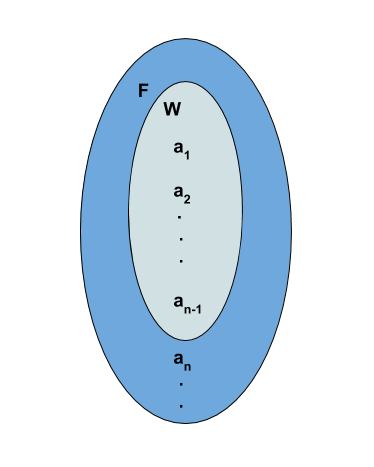
\includegraphics[scale = 0.5]{solutions/3/6/1/b/W_Nullspace.png}
\caption{$\vec{W}$ of dimension n-1, is the null space of $\vec{F}$, where $(a_1,\hdots, a_{n-1})$ are basis vectors for $\vec{W}$}
\end{figure}
\pagebreak
\begin{figure}[h!]
\centering
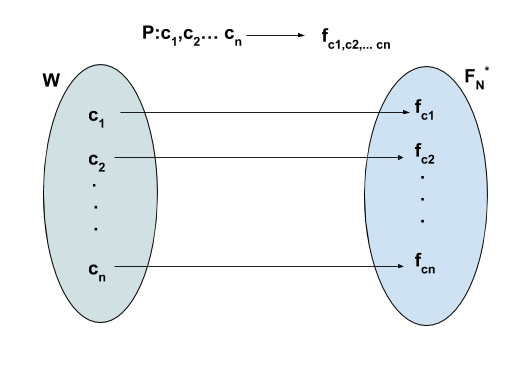
\includegraphics[scale=0.5]{solutions/3/6/1/b/WtoFn.png}
\caption{Mapping from $\vec{W} \xrightarrow{P} \vec{F_N}^*$, where \\ $P(c_1,\hdots,c_n) = f_{c_1,\hdots,c_n}$, $f_{c_1,\hdots,c_n}(x_1, \hdots , x_n) = c_1x_1 + \hdots c_nx_n$} 
\label{fig:1solutions/3/6/1/b/}
\end{figure}
\begin{figure}[h!]
\centering
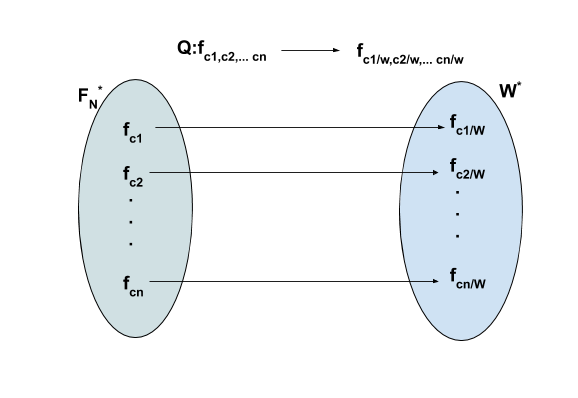
\includegraphics[scale=0.5]{solutions/3/6/1/b/Wdualmap.png}
\caption{Mapping from $\vec{F_N}^* \xrightarrow{Q} \vec{W}^*$, where \\ $f_{c_1,\hdots,c_n}(x_1, \hdots , x_n) = c_1x_1 + \hdots c_nx_n$ is the linear functional with $c_1+\hdots+c_n=0$} 
\label{fig:2solutions/3/6/1/b/}
\end{figure}

\begin{table}[ht]
\begin{center}
\begin{tabular}{|c|c|}
\hline
& \\
Given & $x_1+ \hdots+x_n = 0$ \\
& $(x_1, \hdots , x_n) \in \vec{W}$\\
& $F$ is a field\\
& $\vec{W}^*$ is dual space of $\vec{W}$ \\
& \\
\hline
& \\
To prove & $\vec{W} \xrightarrow{} \vec{W}^*$ is a natural isomorphism\\
& $f(x_1, \hdots , x_n) = c_1x_1 + \hdots c_nx_n$\\
& which satisfy $c_1 + \hdots + c_n = 0$\\
& \\
\hline
& \\
Proof & Let $\alpha_i = \epsilon_1 - \epsilon_{i+1}$ \\ 
& $\quad i \in \{1,\hdots, n-1\}$ \\
& \\
& $\sum_{i=1}^{n-1} c_i \alpha_i = 0$ \\
& $\implies \left(\sum_{i=1}^{n-1} c_i \right) \epsilon_1 - \sum_{i=1}^{n-1} c_i \epsilon_{i+1} = 0$ \\
& $(\alpha_1, \hdots, \alpha_{n-1})$ are linearly\\
& independent and form a basis for $\vec{W}$ \\
& \\
& $\vec{W} \xrightarrow{P} (\vec{F}^n)^* \xrightarrow{Q} \vec{W}^*$ \\
& The function $P$ is defined as \\
& $P(c_1,\hdots,c_n) = f_{c_1,\hdots,c_n}$; where, \\
& $f_{c_1,\hdots,c_n}(x_1, \hdots , x_n) = c_1x_1 + \hdots c_nx_n$ \\
& \\
& Let $Q \circ P (c_1,\hdots,c_n) = 0;$ \\
& $(c_1,\hdots,c_n) \in \vec{W}$ \\
& $Q(f_{c_1,\hdots,c_n}) = 0 \implies f_{c_1,\hdots,c_n|W} = 0$ \\
& $\implies f_{c_1,\hdots,c_n}(x_1, \hdots , x_n) = 0$ \\
& \\
& $f_{c_1,\hdots,c_n}(\alpha_i) = 0; \quad i = 1,\hdots,n-1$ \\
& $\implies c_1 = c_i; \quad i = 2,\hdots,n$ \\
& $\implies \sum_{i=2}^n c_i = (n-1)c_1$ \\
& \\
& since $(c_1,\hdots,c_n) \in \vec{W}$ \\
& $\sum_{i=1}^n c_i = 0$ \\
& $\implies c_1 = 0$ \\
& $\implies c_i = 0 \; ; \quad i = 1,\hdots,n$ \\
& \\
& Hence, $f_{c_1,\hdots,c_n}$ is a zero function. \\
& Thus the mapping $\vec{W} \xrightarrow{} \vec{W}^*$ \\
& is a natural isomorphism \\
\hline
\end{tabular}
\end{center}
\caption{}
\label{table:solutions/3/6/1/b/}
\end{table}
